\documentclass{article}

\usepackage{arxiv}

\usepackage[utf8]{inputenc} % allow utf-8 input
\usepackage[T1]{fontenc}    % use 8-bit T1 fonts
\usepackage{hyperref}       % hyperlinks
\usepackage{url}            % simple URL typesetting
\usepackage{booktabs}       % professional-quality tables
\usepackage{amsfonts}       % blackboard math symbols
\usepackage{nicefrac}       % compact symbols for 1/2, etc.
\usepackage{microtype}      % microtypography
\usepackage{cleveref}       % smart cross-referencing
\usepackage{lipsum}         % Can be removed after putting your text content
\usepackage{graphicx}
\usepackage{natbib}
\usepackage{doi}
\usepackage{subcaption}


\title{Gig-gossip - P2P protocol for the Gig economy}

% Here you can change the date presented in the paper title
\date{February 9, 2023}
% Or remove it
%\date{}

\author{
	{Sonof Satoshi}\thanks{We are the children of Nakamoto} \\
	\href{mailto:sonof.satoshi@donttrustverify.org}{sonof.satoshi@donttrustverify.org}\\
	\href{https://www.Gig-gossip.org}{www.Gig-gossip.org}\\
	Public Key (GPG) of the author~\ref{gpgkey} \\
}

% Uncomment to override  the `A preprint' in the header
%\renewcommand{\headeright}{Technical Report}
%\renewcommand{\undertitle}{Technical Report}
\renewcommand{\shorttitle}{\textit{Gig-gossip} Protocol}

%%% Add PDF metadata to help others organize their library
%%% Once the PDF is generated, you can check the metadata with
%%% $ pdfinfo template.pdf
\hypersetup{
pdftitle={Gig-gossip - P2P protocol for the Gig economy},
pdfsubject={cs.NI,cs.CR},
pdfauthor={Sonof Satoshi},
pdfcreator=,
pdfproducer=,
pdfkeywords={GIG Economy, Gossip Protocol, Distributed System, P2P, Bitcoin, Lightning Network, BTC, LND}
}

\begin{document}
\maketitle

\begin{abstract}
Gig-gossip protocol is a P2P, mobile-first protocol, that enables the decentralisation of the gig economy. It is built on top of Bitcoin financial infrastructure with Lightning Network used for micropayments. It is spam and DDoS protected with its countermeasure on POW (proof of work). Network nodes are financially gratified for enabling prompt communication between parties. Gig dispute resolution is done by payment settlers - organizations that control final payment settlements. Payment settlers are beneficiaries of the integrity of the process and are naturally interested in providing complementary services (like gig worker screening, KYC and making dispute resolution online) that, on the other hand, are beneficial for the quality of service of the proposed decentralised gig economy.
\end{abstract}

% keywords can be removed
\keywords{gig economy \and gossip protocol \and distributed system \and P2P network\and Bitcoin \and Lightning Network}

\section{Motivation}
The gig economy refers to the work done by casual workers coordinated by a software system. At the time of this writing, the end customer of the gig economy interacts with a centralized, cloud-based platform (app). This platform is also used to pay for the services after the job is done to the platform, which in turn is sharing the revenue with the assigned gig worker. The actual job is done by the gig worker for their customer, making the online platform a tool that supports and manages the effectiveness of the job.

This kind of cybernetic system uses the human power of gig workers managed by AI, to extract value for the company shareholders. The AI component of the platform uses behavioural data represented as all the user (both gig workers and customers) interactions with the platform to maximize the total revenue generated by the system and the underlying company that operates it. To optimise the global goal, which is the company revenue, the platform is implementing gamification and for-purpose misinformation techniques. It is possible because gig workers and customers have no other option but to trust the platform for its efficiency and the underlying operation of the platform is opaque to users and configurable only by the operating central company. Therefore the platform operator:

\begin{enumerate}
\item dictates the revenue sharing and can change this anytime dependingly on the socioeconomic circumstances without giving any reason to gig workers
\item punish workers that are not behaving properly, meaning that their behaviour is not aligned with the company benefit, and doing it e.g. by blocking them from access to the platform
\end{enumerate}

We are proposing a P2P protocol designed for the gig economy that, by eliminating the need for central online platforms, will create a new decentralized, P2P gig economy (Figure \ref{fig:decent}). Gig workers will be engaged directly by the end customer and can accomplish their tasks and earn money on a free market without the need for the existence of a central organization. Quality of service delivery and conflict resolution is preserved by payment settlers - companies that earn their revenue by assuring compliance consistency of the system - the ability to maintain compliance with all relevant laws, regulations, and standards consistently over time. 

The lack of central organization also means that minimal data is shared between gig workers customers and payment settlers. Just enough to fulfil the job according to the protocol-driven off-chain smart contract that uses P2P money i.e. Lightning Network \cite{poon2016bitcoin} on Bitcoin \cite{nakamoto2009bitcoin}, therefore forming layer 3 protocol from the Bitcoin perspective.

\begin{figure*}[t!]
    \centering
    \begin{subfigure}[t]{0.4\textwidth}
        \centering
        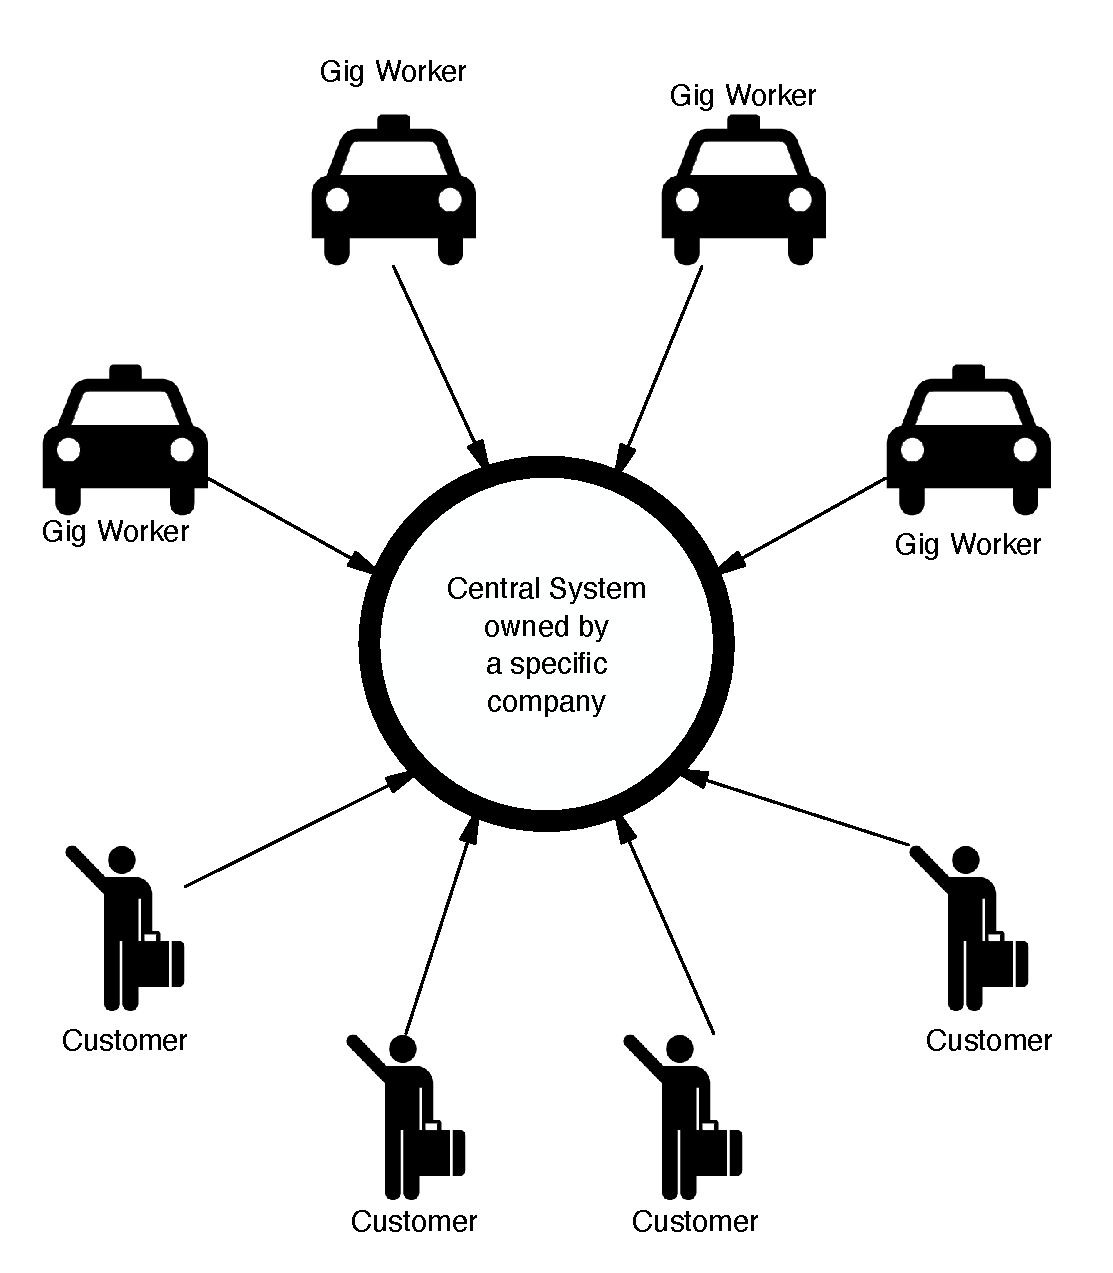
\includegraphics[scale=0.25]{centralised.pdf}
        \caption{Centralised system}
    \end{subfigure}%
    ~ 
    \begin{subfigure}[t]{0.4\textwidth}
        \centering
        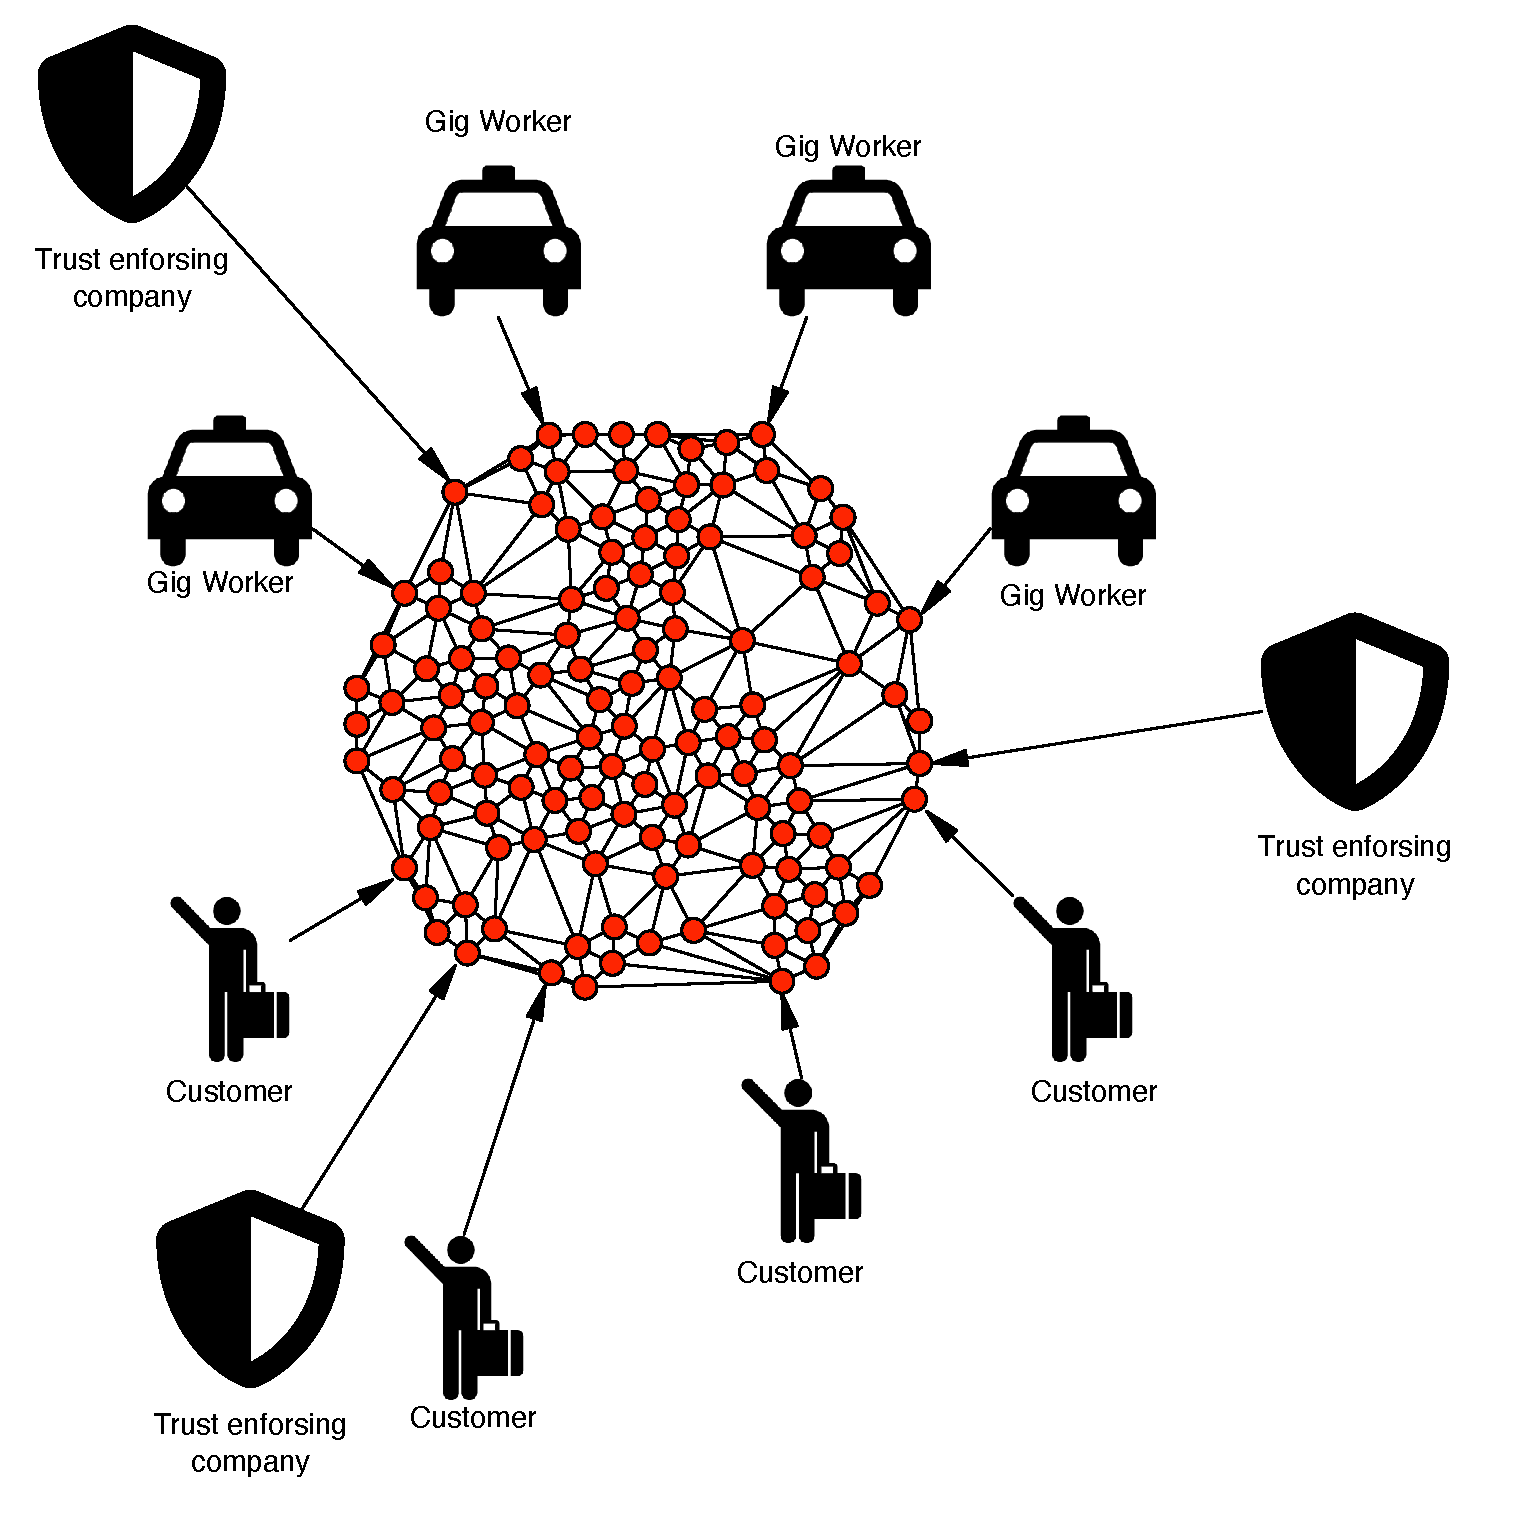
\includegraphics[scale=0.25]{decentralised.pdf}
        \caption{Decentralised system}
    \end{subfigure}
    \caption{Centralised vs Decentralised Gig-economy}
	\label{fig:decent}	
\end{figure*}

\section{Gig-gossip P2P Network}
Gig-gossip P2P Network is a globally symmetric, P2P network, meaning that there is no direct need to run any operation critical services in the cloud or any other centralised computing environment, you just need your mobile phone. In other words, Gig-gossip node is a software module that is run by every device that uses Gig-gossip protocol and it forms a basis of communication. Moreover, Gig-gossip nodes can be implemented as apps and run efficiently on cheap modern mobile devices. 

We are not inventing any new coin or crypto token, but rather we are speaking about the way how Gig-gossip protocol forms a layer 3 protocol on top of the Lightning Network (being itself a layer 2 network sitting on top of the Bitcoin network), therefore the Bitcoin is a native token of the Gig-gossip network.

Gig-gossip P2P network preserves:
\begin{itemize}
\item P2P Symmetry - every node does the same thing
\item Permissionlessness - anyone with internet access can join Gig-gossip P2P network
\item Mobile first - the cost of running a Gig-gossip node is marginal on modern mobile devices. 
\item Privacy - the communication is encrypted
\item Anonymity - any sensitive information about the people behind the nodes is encrypted
\item DDos and Spam protection - it uses POW (proof of work) as a countermeasure for DDoS and Spam
\item Sustainability - the protocol is designed so that honest participants are more beneficial than unhonest ones implementing the implicit punishment principle
\end{itemize}

Gig-gossip Protocol is a gossip protocol \cite{Fanout}, that allows a network to broadcast messages in a similar way to gossip spreads. Assuming that each Gig-gossip node is connected to its peers and that the network graph is connected, each node works independently and in the event of receiving a message that needs to be broadcasted it spreads it to its peers (Figure~\ref{fig:network}). 

Gig-gossip is a protocol, meaning that it only specifies a minimal set of rules. It doesn't say explicitly how the network node should be implemented. The node implementation is free to do whatever is best and beneficial for the node owner.

\begin{figure}
	\centering
	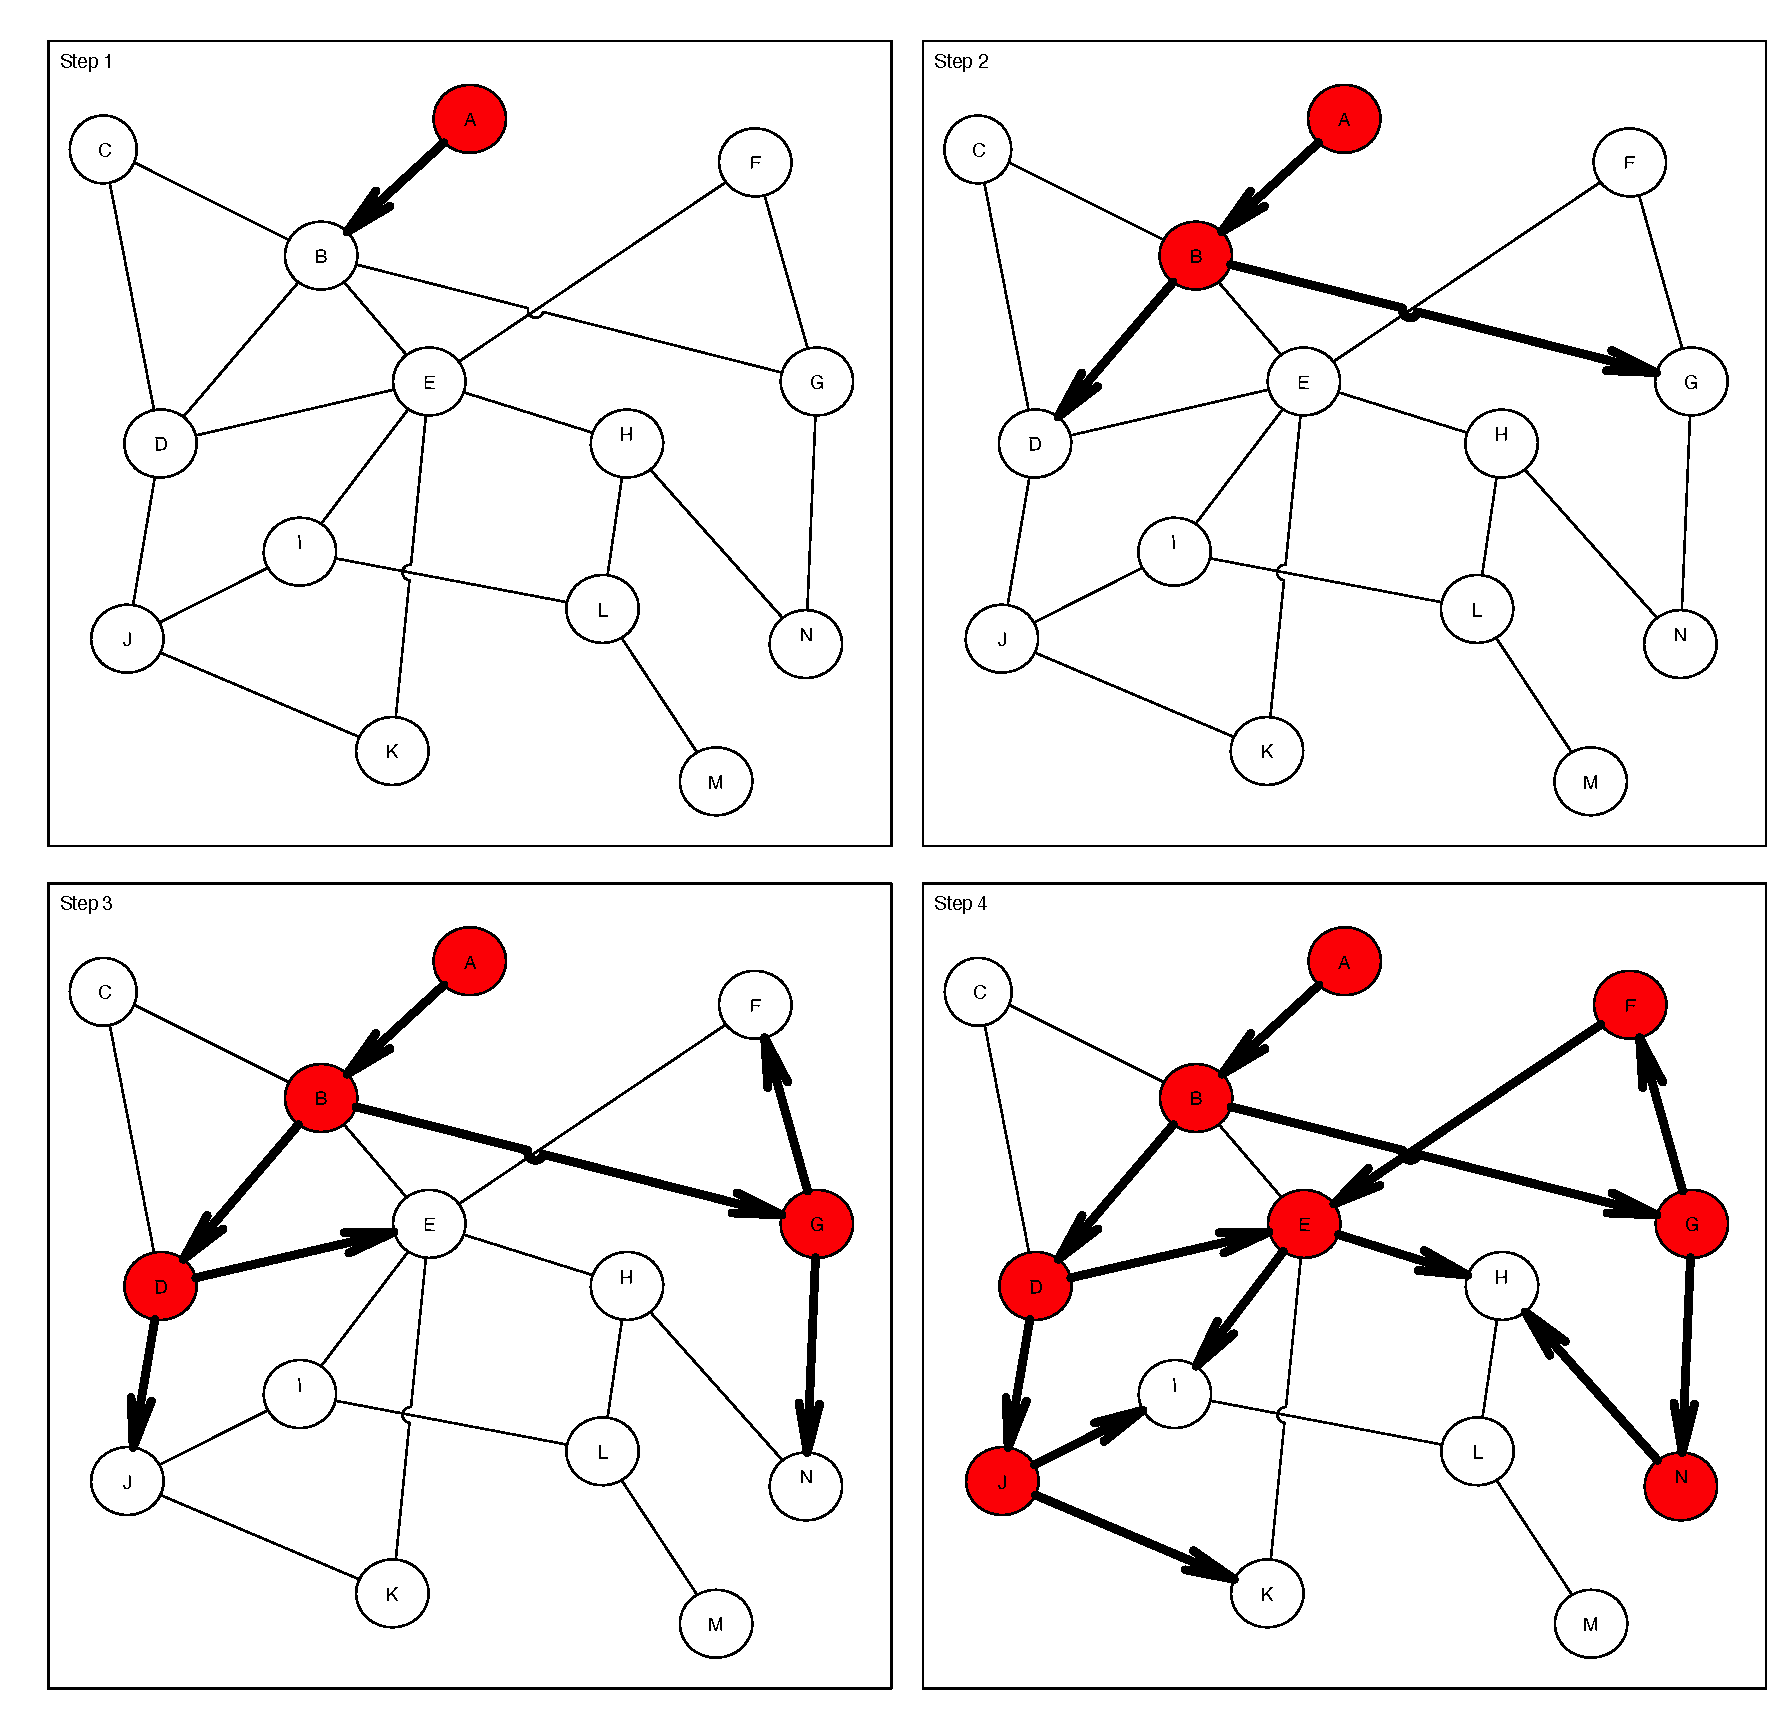
\includegraphics[scale=0.4]{network.pdf}
	\caption{The intuition behind gossip protocol}
	\label{fig:network}
\end{figure}

\subsection{Payment settler as the compliance consistency enforcer}
Every gig economy environment needs to maintain safety understood as protection from fraudulent activities during service delivery, either if it is a taxi ride, delivering food or programming a website. Gig-gossip has built-in tools for the countermeasure for activities like:
\begin{enumerate}
	\item Incompetence of the gig worker that can result in physical/financial harm to the customer
	\item Making sure that the customer has money to pay the gig worker before the service is provided
	\item Disputes between customer and gig worker
	\item Criminal acts associated with the service delivery that require law enforcement actions
	\item Terrorism funding
\end{enumerate}

Gig-gossip brings the building blocks for the institutions that directly benefit from the compliance consistency of the system:
\begin{enumerate}
	\item Digital certificates - the way how gig workers can prove their competencies. It also enables KYC allowing for dispute resolutions and counterterrorism actions 
	\item HODL invoices - the Lightning Invoices that require settlement of the payment implementing Authorisation Hold on the customer side, making sure that the customer has the money but the payment settler controls the final settlement and preventing terrorism funding.
\end{enumerate}
 
\section{The protocol}
The core task of Gig-gossip protocol is to broadcast a job proposal (topic) to interested parties and collect job offers (reply messages) from interested contractors. Economically, the customer is interested in exchanging their money for the service, while gig worker is interested in being paid for the job done. The network to sustain its existence needs to reward broadcasters for the quality of the broadcasting. Therefore the protocol is constructed in a way that the customer broadcasts a topic, that contains an anonymous job description. This job description is delivered by the network to the gig worker that is happy to respond with an encrypted message that is targeted solely to the customer. The message is delivered back to the customer that can verify the basic properties of the gig worker with their digital certificate but to decrypt the contact information allowing for further P2P communication with the gig worker, the customer is obligated to pay the network and lock the required amount of money proposed in the job offer. The payment settlement is secured by payment settlers - companies that secure compliance consistency of the system.

For clarity, we use the following naming convention:

\begin{enumerate}
	\item Topic - the job proposal broadcasted through the network
	\item Reply Message - the job offer for a specific topic sent from the contractor
	\item Peer - any gossip network node. Every peer maintains a list of their peers.
	\item Sender - Peer that is the source of the topic. From the gig economy point of view, it is a customer.
	\item Originator - Peer that is currently broadcasting the topic to its peers.
	\item Middleman - Peer that is passing the broadcasted topic further as well as bringing back the reply message
	\item Replier - Peer that is replying to the broadcasted topic with a reply message.
	\item Settler - the specific payment-settler
\end{enumerate}

Here, we assume that nodes of the Gig-gossip network are already connected to their peers via some internet transport protocol (e.g. TCP, UDP with or without hole punching \cite{WebRTC}, mobile mesh etc.) and all the peers are accepting Gig-gossip protocol. How the nodes discover their peers is not a part of the protocol.

In short, the Gig-gossip protocol can be summarised as follows:

\begin{enumerate} 
	\item  \textbf{Asking for broadcast} If the originator wants to broadcast the topic the first step is to ask its peer (the middleman) about the condition on which the peer is happy to broadcast the specific topic. If the middleman accepts this kind of topic, it replies to the originator with specific POW properties the originator needs to compute to be able to broadcast the topic by this middleman.
	\item  \textbf{Broadcast with POW:} In order to use this middleman the originator must compute a hash (e.g. SHA256) that is less or equal to the specific target for the specific POW scheme. The computed POW is passed with the topic to the broadcaster and if the broadcaster validates the hash it broadcast the topic to its peers.
	\item  \textbf{Replying:} If instead, the middleman is interested in accepting the job it becomes the replier. Replier constructs the reply message. The reply message has to be encrypted by the selected payment settler. The message is then passed back to the sender by the network. The reply message contains all the information that is required to pay for the reply message delivery to all the middlemen involved. 
	\item  \textbf{Paying for the reply message:} Once the message reaches the sender, the sender needs to pay the network to obtain the key allowing for message description. The payment here is not settled until the payment settler reveals the key and can be revoked by the payment settler. 
	\item \textbf{Payment settlement:} The payment is settled by the payment settler and the settlement of the payment involves also the payment to the network. Once, the payment settler reveals the key the originator can begin direct communication with the replier. The payment settlement of the money required to pay for the gig is delayed until the job is done and all the disputes are resolved.
\end{enumerate}

\subsection{Topic}

The topic is a data structure that defines the basic requirements for the job. It is application specific and by design, it should not reveal any information about senders allowing for their identification.

Let's use a taxi app as an example {Figure~\ref{fig:fr:topic}}. The topic of this taxi app has a form of two geo-hashes and time intervals describing from where and when the ride can be executed. Geo-hash here is a way of encoding a specific geographical place (a geographical cell that has a form of rectangle) in a form of a string where the length of the geo-hash determines its precision.

\begin{figure}
	\centering
	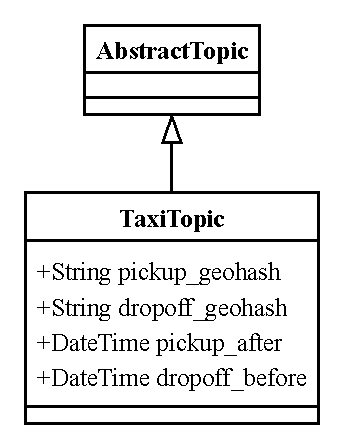
\includegraphics[scale=0.7]{Topic.pdf}
	\caption{The topic frame}
	\label{fig:fr:topic}
\end{figure}


For example, Legal Services Council in Sydney is located at the following coordinates latitude= -33.8647 and longitude=151.2096 and the corresponding geo-hash of precision 7 is equal to `r3gx2g5`.

The precision of geo-hash determines the size of the cell (Table~\ref{tab:geoprec}) and to be useful for the taxi app it needs to be at least 7 so the cell has a size lower than 200m (see table below)

\begin{table}
	\centering
	\begin{tabular}{lll}
		\toprule
		Geo-hash length & Cell width & Cell height \\
		\midrule
		1  & $\le$ 5,000km & $\times$ 5,000km \\
		2  & $\le$ 1,250km & $\times$ 625km   \\
		3  & $\le$ 156km   & $\times$ 156km   \\
		4  & $\le$ 39.1km  & $\times$ 19.5km  \\
		5  & $\le$ 4.89km  & $\times$ 4.89km  \\
		6  & $\le$ 1.22km  & $\times$ 0.61km  \\
		7  & $\le$ 153m    & $\times$ 153m    \\
		8  & $\le$ 38.2m   & $\times$ 19.1m   \\
		9  & $\le$ 4.77m   & $\times$ 4.77m   \\
		10 & $\le$ 1.19m   & $\times$ 0.596m  \\
		11 & $\le$ 149mm   & $\times$ 149mm   \\
		12 & $\le$ 37.2mm  & $\times$ 18.6mm  \\
		\bottomrule
	\end{tabular}
	\caption{Geo-hash precision}
	\label{tab:geoprec}
\end{table}

On the other hand, we do not want to be too specific and we might want to restrict the size of geo-hash to at most 8, so it is not possible to precisely locate the originator (customer) at this stage, but on the other side, the precision is enough for the taxi driver to accept/reject to the job.
Network nodes will prefer to make the exact position confidential at the moment of broadcast, therefore they might not accept locations in taxi-topicks that are too specific.

\subsection{Digital Certificates}
Digital Certificates are the way to implement gig worker screening and KYC. For the internet public-key infrastructure (e.g. X.509 certificates \cite{x509} ) these certificates are issued by certification authorities that can be either trusted 3rd parties or communities. For a taxi driver, the screening requires having a valid driving licence and no criminal record. The payment settler can issue this kind of certificate by signing it with its private key so anyone can verify that the specific certificate was truly issued by the issuing organization. If the certificate is revoked the information about it is published by the issuing organization in form of a revocation list. Public key certificates usually contain also a public key of the certified person (Figure \ref{fig:fr:certificate}), so it is possible to use it to encrypt a message that is targetted for this person and verify their signatures.

\begin{figure}
	\centering
	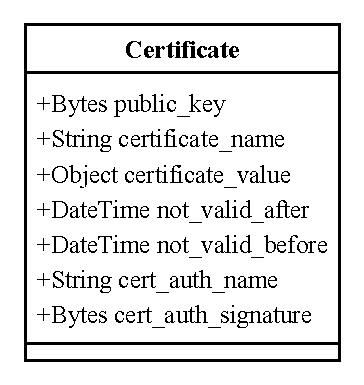
\includegraphics[scale=0.7]{Certificate.pdf}
	\caption{The digital certificate}
	\label{fig:fr:certificate}
\end{figure}

\subsection{Asking For Broadcast}
The first step of Gig-gossip protocol is to send the AskForBroadcastFrame (Figure \ref{fig:fr:askforbroadcast}) to the potential broadcaster.

\begin{figure}
	\centering
	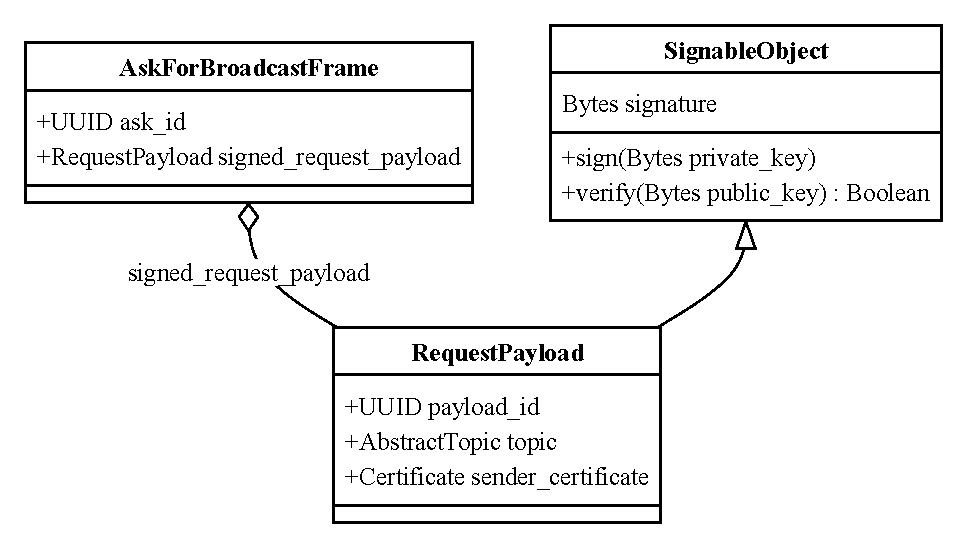
\includegraphics[scale=0.7]{AskForBroadcast.pdf}
	\caption{The AskForBroadcastFrame}
	\label{fig:fr:askforbroadcast}
\end{figure}

AskForBroadcastFrame contains ask\_identifier and digitally signed RequestPayload. Signed RequestPayload is made of unique payload\_id, topic (e.g. TaxiTopic), sender\_certificate and sender signature obtained by signing the RequestPayload with the sender private key that is complementary to the public key stored within the sender\_certificate. Anyone can verify the RequestPayload by validating its signature with the sender's public key from the certificate. The sender's certificate can always be verified using the public key of the payment settler and checking its published revocation list. The sender's certificate can be issued after KYC, by the organization responsible for dispute resolutions.

Ask\_identifier identifies the frame during the originator-middleman ping-pong communication (Figure \ref{fig:fr:pingpong}). In the gossip protocol, the same broadcasting message may hit the same gossip node many times, so payload\_id is to remain a unique identifier that allows one to determine this situation and react accordingly to the node policy. Some nodes might wish not to broadcast the RequestPayload more than once, others if working on small fanout might wish to broadcast the same RequestPayload many times. Anyway, it is the requested responsibility to ensure the uniqueness of payload\_id, risking that if it is not unique it will be lost during the broadcast as other nodes can decide that it was already broadcasted if the payload\_id was already seen before.


\begin{figure}
	\centering
	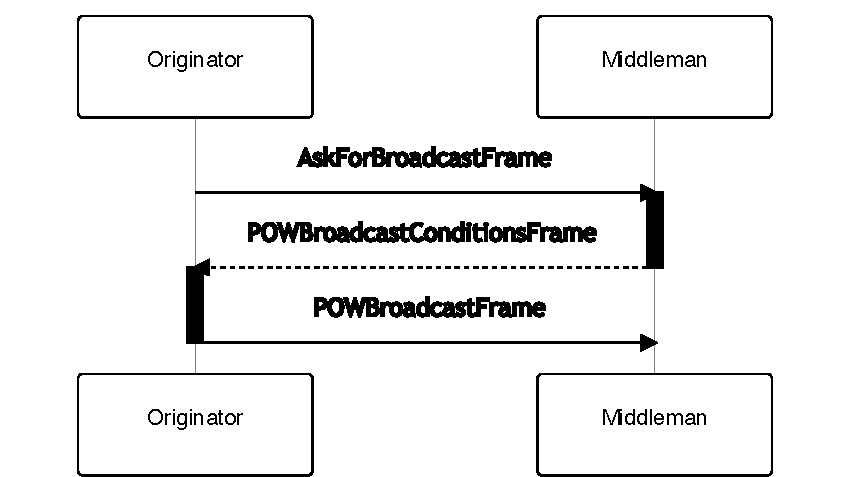
\includegraphics[scale=0.7]{PingPong.pdf}
	\caption{Ping Pong communication sequence}
	\label{fig:fr:pingpong}
\end{figure}

\subsection{Proof Of Work (POW)}
Message broadcast in Gig-gossip is protected with the idea of Proof of Work. POW was introduced in HashCash \cite{Hashcash} and famously implemented in bitcoin mining but was originally introduced to limit email spam. The thinking here is that if the originator needs to make some significant computation to be able to send the message it will significantly increase the cost of spam and DDoS attacks. 

There are many possible POW schemas (e.g. SHA hash-based POW, similar to the one implemented in the bitcoin network \cite{nakamoto2009bitcoin}). In Gig-gossip, given the topic, the middleman decides the kind and how complex POW is required to be computed by the originator to allow further spreading of this topic. For example in the case of hash-based POW, the task is to compute the hash of the specific payload so the hash itself is lower or equal to a specific target. The larger target is the more complex and costly the computation is. On the other hand, once the hash is computed, it is easy to verify that it fits into the specific target, so the broadcaster has an easy task to verify that the originator has done the work to compute the correct hash.

\subsection{Onion-routing}
Gig-gossip is using the onion-routing technique to hide the message reply route (the route that the replies go from the replier to the sender) from the participating middlemen. During the broadcast phase, the onion grows layer by layer. Active peer appends its address to the onion and is using the public key of the next peer to encrypt the grown onion, therefore only the next peer can decrypt that layer of the onion. Once encrypted the onion is passed to the next peer.

\begin{figure*}[t!]
    \centering 
    \begin{subfigure}[t]{0.3\textwidth}
		\centering
		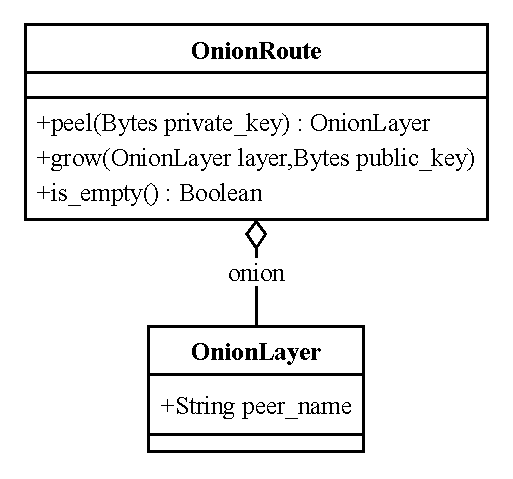
\includegraphics[scale=0.7]{OnionRoute.pdf}
	\end{subfigure}%
    ~ 
    \begin{subfigure}[t]{0.7\textwidth}
		\centering
		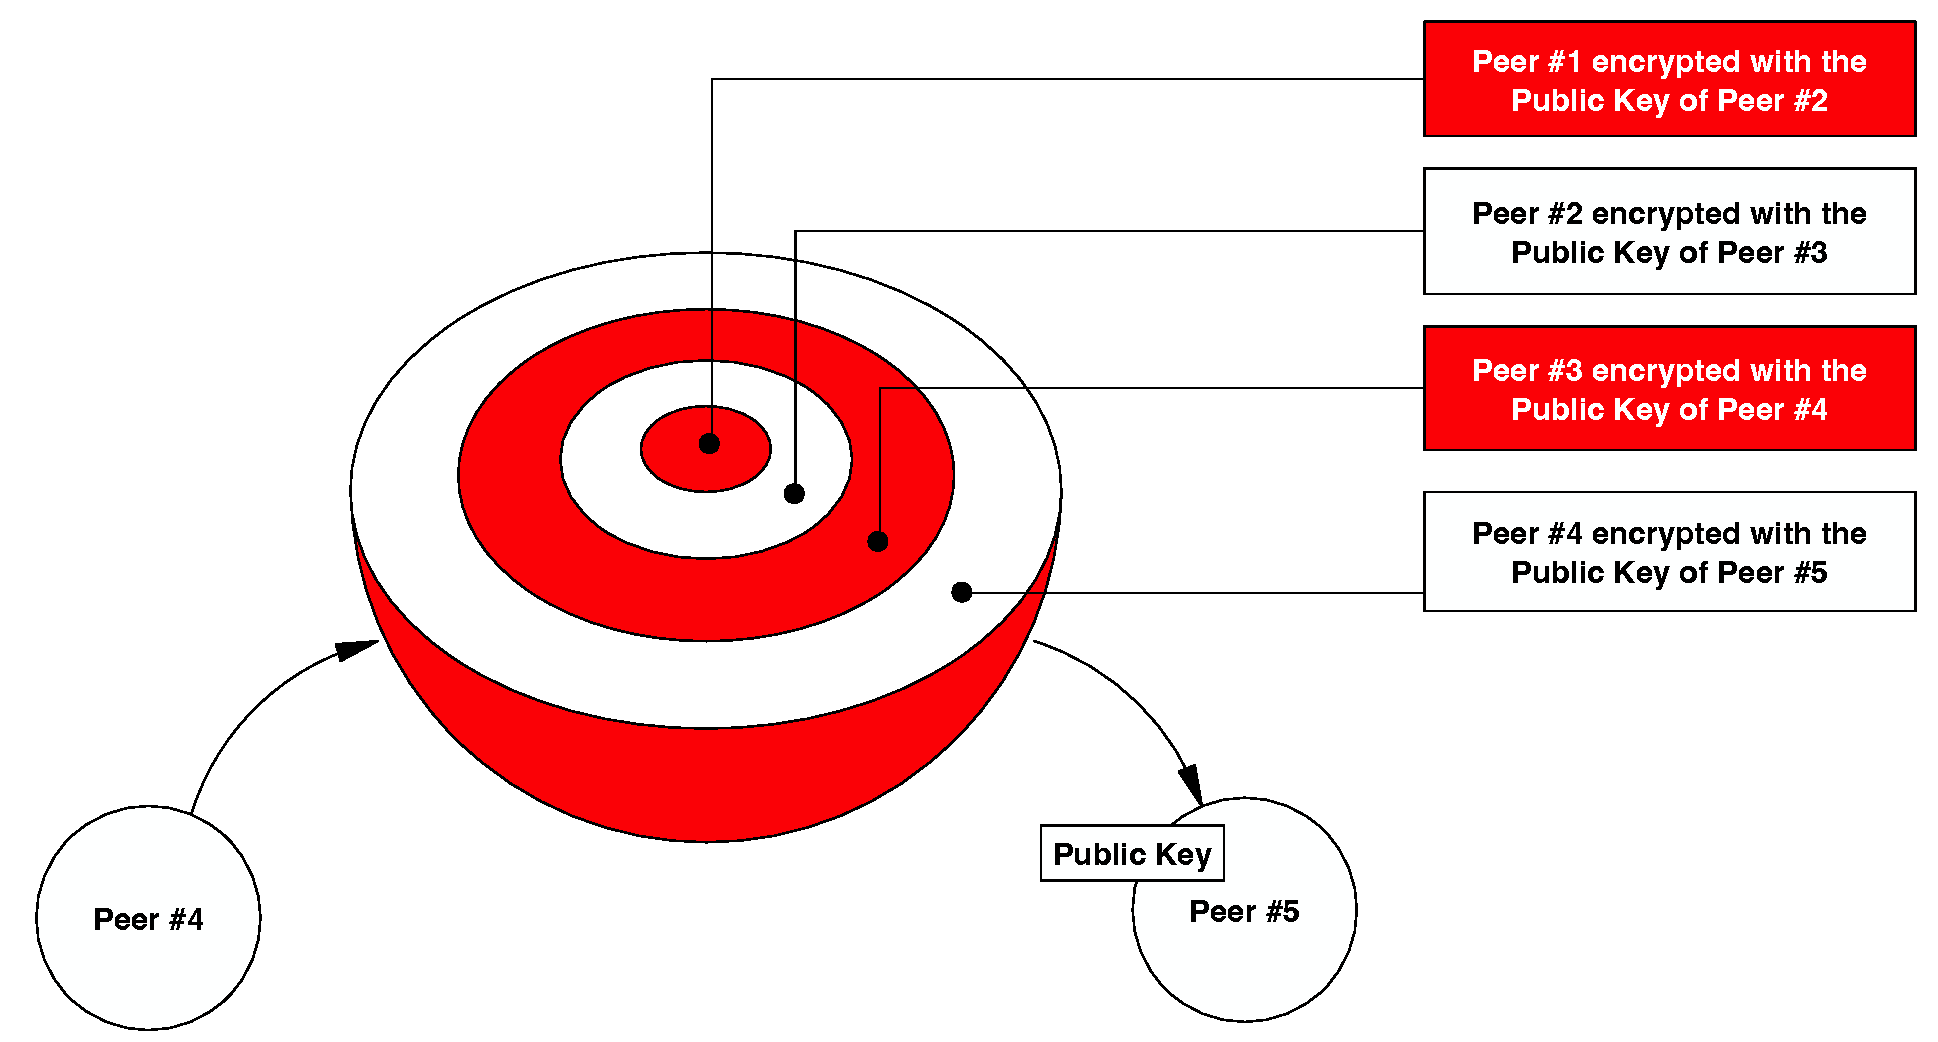
\includegraphics[scale=0.35]{onion.pdf}
	\end{subfigure}
    \caption{Onion-routing}
	\label{fig:fr:onionrouting}
\end{figure*}


This way of constructing the onion allows peeling the onion back to the sender through the network in a way that none of the nodes knows the sender nor the distant peers.

\subsection{Broadcast with POW} 

If the middleman accepts the topic specified in the AskForBroadcastFrame, it sends back the POWBroadcastConditionsFrame (Figure \ref{fig:fr:pingpong}). This frame describes the properties of POW expected to be computed by the originator and payment instructions expected by the peer for delivering the reply.

Starting with ask\_id, which matches with AskForBroadcastFrame, and valid\_till timeout meaning that the middleman will wait only till the specific time for the POWBroadcastConditionFrame (Figure \ref{fig:fr:powbroadcastcondition}) from the originator, it contains also WorkRequest that describes properties of POW and, to prevent reusing POW the timestamp\_tolerance is sent. Timestamp\_tolerance is the maximal time distance from the timeout that is accepted by the broadcaster.

\begin{figure}
	\centering
	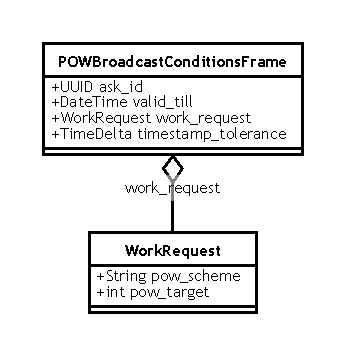
\includegraphics[scale=0.7]{POWBroadcastCondition.pdf}
	\caption{POWBroadcastConditionsFrame}
	\label{fig:fr:powbroadcastcondition}
\end{figure}

The originator is replying to it with POWBroadcastFrame which is also marked with the corresponding ask\_id. The main part is a broadcast\_payload that contains the original signed\_request\_payload (the one that was a part of AskForBroadcast and was already signed by the originator) and backward\_onion that implements the onion routing.

POWBroadcastFrame also contains ProofOfWork that contains a hash value (nuance) that fits below pow\_target for the specific pow\_scheme and was computed as a hash of broadcast\_payload part, therefore middleman can easily verify nuance value by computing the hash of broadcast\_payload and checking if it is lower or equal to the pow\_target. 

Additionally, POWBroadcastFrame contains the timestamp that makes the frame POW impossible to use after the timestamp\_tolerance is reached. In other words, the following must hold:

\begin{center}
	timestamp$\le$ \textbf{now}$\le$ timestamp+timestamp\_tolerance
\end{center}

\begin{figure}
	\centering
	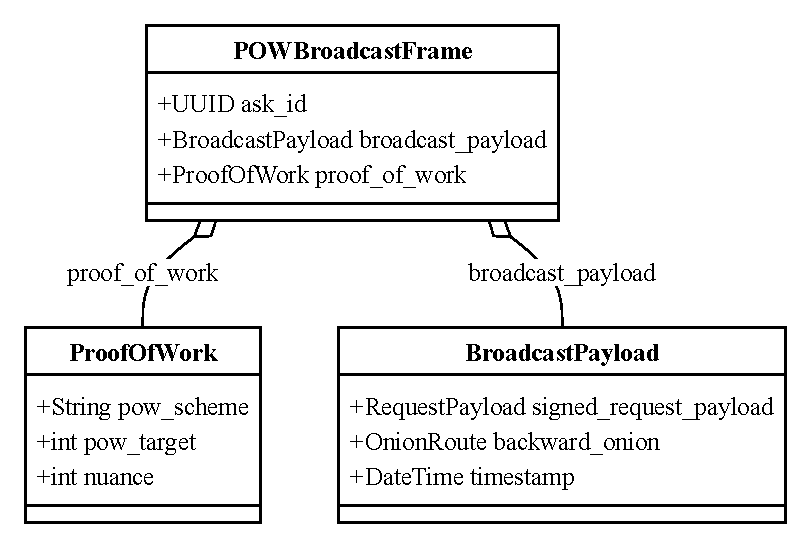
\includegraphics[scale=0.7]{POWBroadcastFrame.pdf}
	\caption{POWBroadcastFrame}
	\label{fig:fr:powbroadcastframe}
\end{figure}

Each step of the broadcast involves passing a specific BroadcastPayload that consists of RequestPayload that is never changed and protected by the cryptographic signature.  Additionally, every BroadcastPayload adds a new layer to the backward\_onion.

In the gossip protocol nodes are randomly selected from the list of all the known peers of the originator. This number is sometimes referred to as fanout \cite{Fanout} of the gossip protocol. Once selected the broadcasting process is performed.

It's important to notice that while in vanilla gossip we are focused on making sure most of the nodes have retrieved the message, in Gig-gossip it is beneficiary for the network to build multiple routes that will provide the customer with a way to choose the one that has the minimal network fee. Therefore, here we allow for multiple crossing of the same node with the same topic on purpose, being a decision made by the node owner.

\begin{figure}
	\centering
	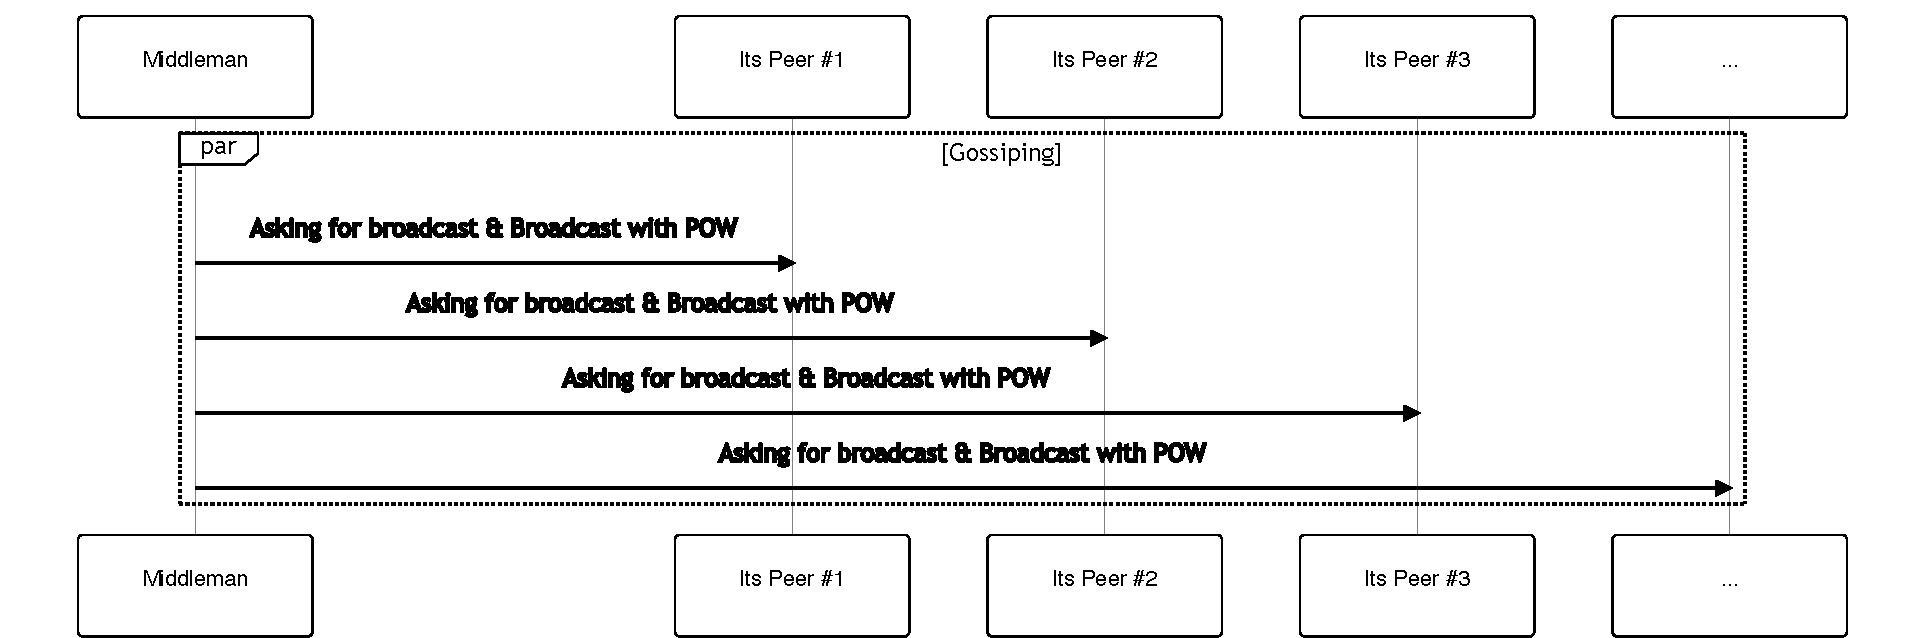
\includegraphics[scale=0.8]{BroadcastSequence.pdf}
	\caption{Broadcast Sequence}
	\label{fig:fr:broadcastsequence}
\end{figure}

\subsection{Lightning Network, HODL invoices, payments, preimages and payment-hashes}

Lightning Network is a layer 2 network built on top of the Bitcoin network that allows for cheap and fast micropayments. It is built around the concept of channels. Once the channel is opened (that usually means funding it with some amount of Bitcoin), it can be used to issue and pay the invoice. Payment generates proof. 

The interesting kind of invoices implemented in Lightning Network is HODL invoices. This idea extends the invoice-payment process with the cryptographic concept of preimage for payment hash in the following way:
\begin{enumerate}
	\item Invoice is issued by the issuer and it contains a specific payment hash. Payment hash is a hash of preimage that itself is a number known only to its creator, that in the case of HODL invoices is usually a different actor: a settler. The payment hash is the only thing that is exposed on the invoice.
	\item Payer is paying the HODL invoice under the condition of having the preimage published. In other words, the payment means that the invoice is paid if the preimage is revealed and that this preimage has the payment hash that was presented on the invoice. Once paid the invoice is called Accepted.
	\item Accepted invoice is Settled once the preimage is revealed.
\end{enumerate}


\begin{figure}
	\centering
	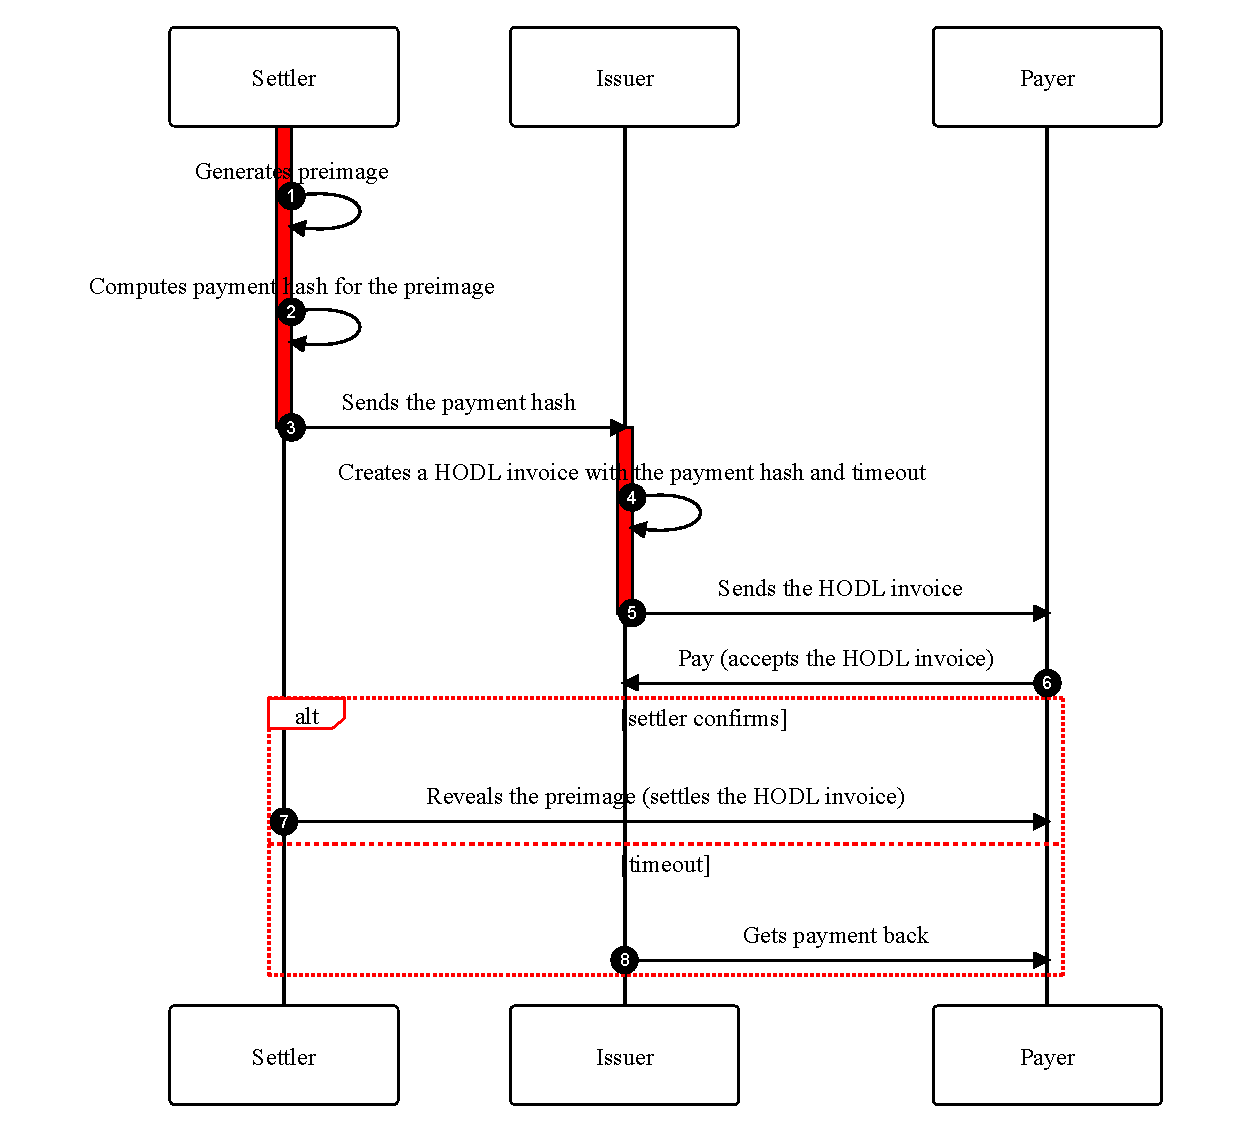
\includegraphics[scale=0.6]{LNDSequence.pdf}
	\caption{Lightning Network HODL Invoice Sequence}
	\label{fig:fr:lndsequence}
\end{figure}

\subsection{Cryptographic Payment Chains base on HODL invoices}
A cryptographic key can be used as a preimage for generating a payment hash for the invoice. Such a key might allow the description of the specific encrypted message. In other words, having a message that is encrypted with a specific key we can construct an invoice using the key as a preimage and compute its payment hash. To decode the message payer needs to pay the invoice and the key (preimage) needs to be revealed by the settler (that will settle the payment).

We can create a chain of issuers that are becoming middlemen between the payer and settler (Figure \ref{fig:cryptopaychain}). The settler generates the preimage (cryptographic key) and uses it to encrypt the specific message that is revealed to the public. The settler issue the invoice containing the payment hash for the generated preimage. Issuers in the chain, one after another are generating HODL invoices using the same payment hash received from the settler. Once the payer is reached and the payer pays the invoice and this triggers the chain of payments that eventually reaches the settler. The settler reveals the preimage making the payment settlement and the preimage being the key allows to decode the message. In other words, the HODL invoice ensures all the issuers that the payment was made (invoices are in the accepted state) but to have control of the money, they need to use the preimage, so all the chain needs to see the preimage, therefore they are forced to pay invoices of their peers. Once the last invoice is paid to the settler, the settler reveals the preimage and all the invoices are settled at the same time. Also as the preimage = key, the message can be decoded.


\begin{figure}
	\centering
	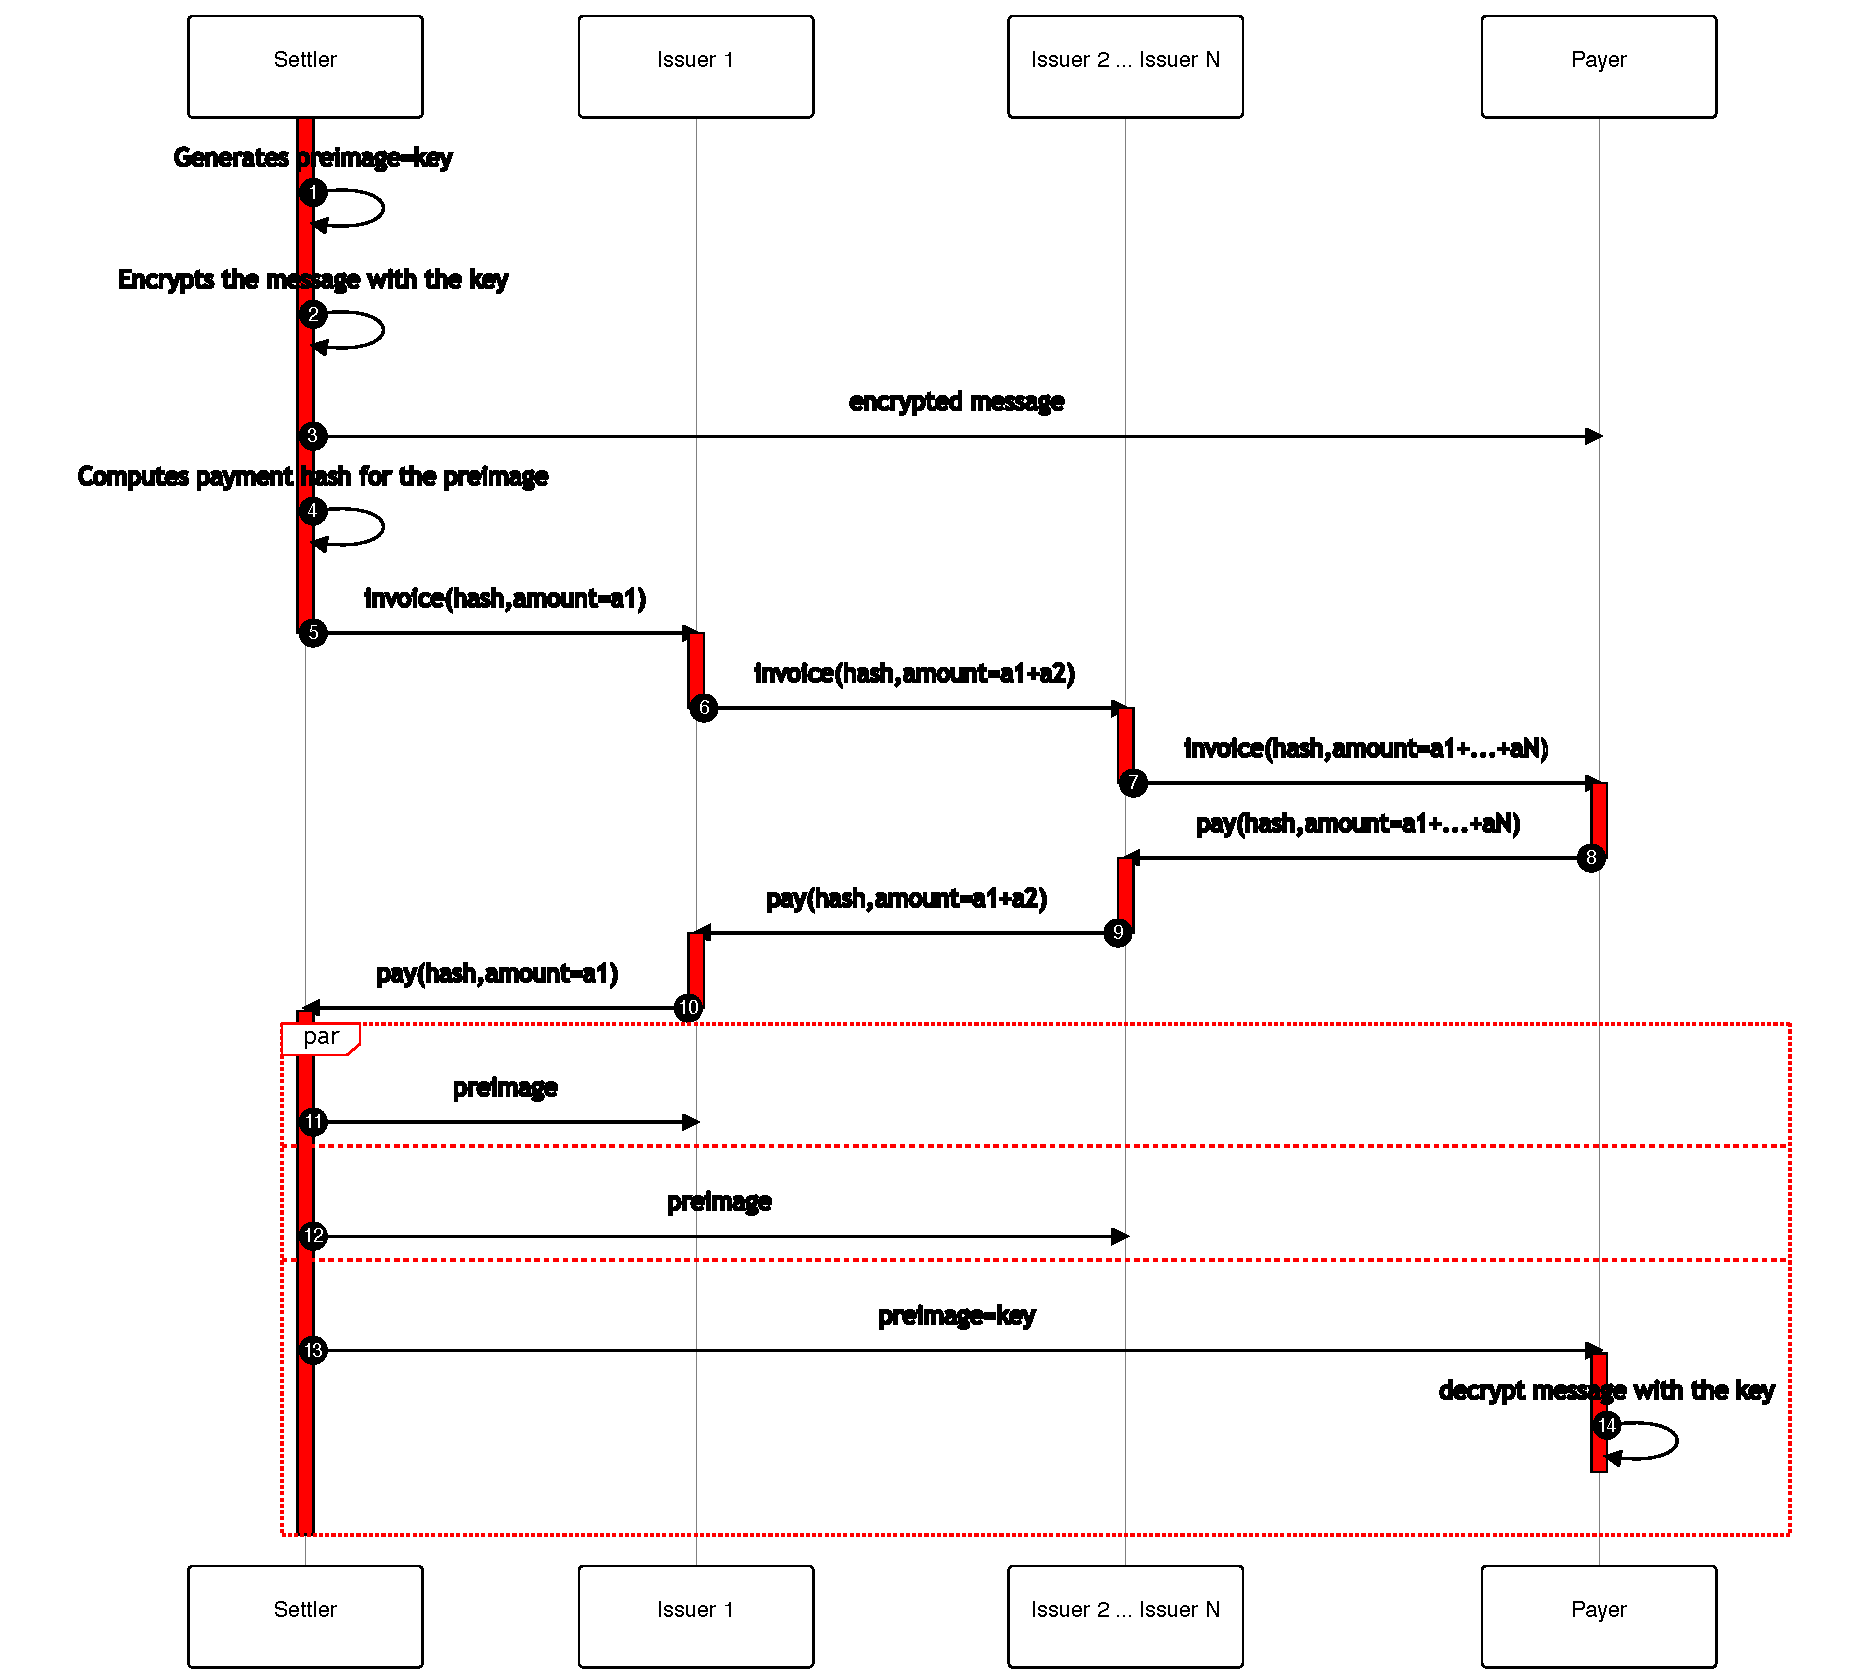
\includegraphics[scale=0.7]{PaymentChain.pdf}
	\caption{Cryptographic Payment Chain Sequence}
	\label{fig:cryptopaychain}
\end{figure}

There are two issues with this scheme that make the payment settler an entity that manages the trust in the cryptographic payment chain:
\begin{enumerate}
	\item The preimage = key corresponds to the encrypted message, but it is not possible \footnote{This can be solved in the future by zk-snark \cite{zksnark} } to see that just looking at the payment hash and the encrypted message, therefore all the issuers and the payer need to trust the settler that he has encrypted the message with the specific preimage, that corresponds to the payment-hash on all the invoices.
	\item Preimage must be revealed only \textbf{after} the settler receives the payment. If for some reason the settler decides to reveal the preimage=key before receiving the payment the payer does not need to pay the invoice, as the key was already revealed, and therefore no one in the chain will be paid.
\end{enumerate}


\subsection{Replying}
The node (replier) that is happy to accept the job described in the topic, instead of broadcasting it further is replying with ReplyFrame which is sent back over the Gig-gossip network to the node that was the sender of the topic. The replier needs to specify its price for the required service and can send the encrypted message to the sender. This message should contain all the details allowing for further P2P communication between the sender and the replier (e.g. replier's IP address).

The replying sequence is illustrated in Figure \ref{fig:replyandpay} and \ref{fig:payforservice}. 

The replier starts with constructing a ReplyPayload. This payload contains replier\_certificate, signed\_request\_payload and encrypted\_reply\_message.

The replyier\_certificate allows the sender of the topic to identify that the gig worker is a credible service provider by checking the certificate and verifying its "hard" certification (e.g. driving licence) with the specific certification authority being a trusted third party (e.g. government agency or specialised certification verifier)

The signed\_request\_payload is sent back to the sender allowing for verifying that the topic is the same as the one that was sent by the sender and that no one has modified it. 

The encrypted\_reply\_message is the message that is encrypted with the sender public\_key that is a part of the sender's certificate in the signed\_request\_payload, so only the sender can read it.

The payment settler will generate the preimage and will use this preimage to encrypt the ReplyPayload and generate a network\_payment\_hash for the cryptographic payment chain. Payment settler returns the SettlementPromise to the replier, being itself a set of hashes and certificates allowing use by the Gig-gossip network node to verify the correctness of the ReplyFrame. One of them is the hash\_of\_encrypted\_reply\_payload. The other is the network\_payment\_hash used in all network invoices. SettlementPromise is signed by the settler and contains the settler\_certificate, which allows verification of the specific settler.

At the same time, the replier needs to ask the settler about the payment hash of the main reply\_invoice (Figure \ref{fig:payforservice}). The reply\_invoice is the invoice that must be used by the sender to pay for the service. 

Another field of the ReplyFrame is the forward\_onion that starts as a copy of the backward\_onion, and then each of the middlemen is peeling one layer of the onion, using its private key and sending it to the node that is found there in the peel.

\begin{figure}
	\centering
	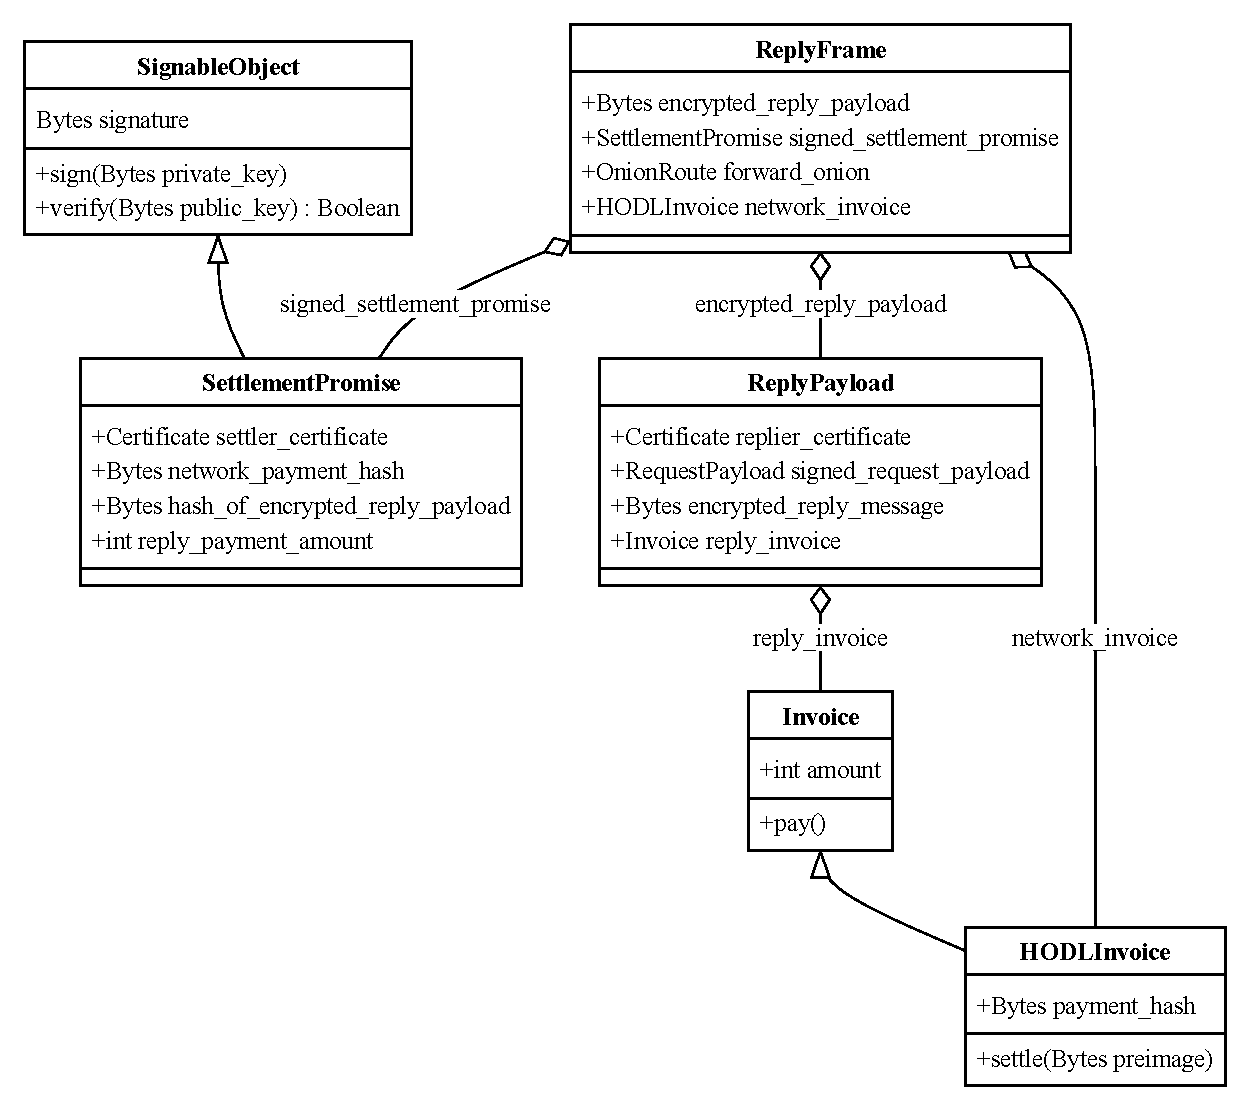
\includegraphics[scale=0.7]{ReplyFrame.pdf}
	\caption{Reply Frame}
	\label{fig:fr:replyframe}
\end{figure}

\begin{figure}
	\centering
	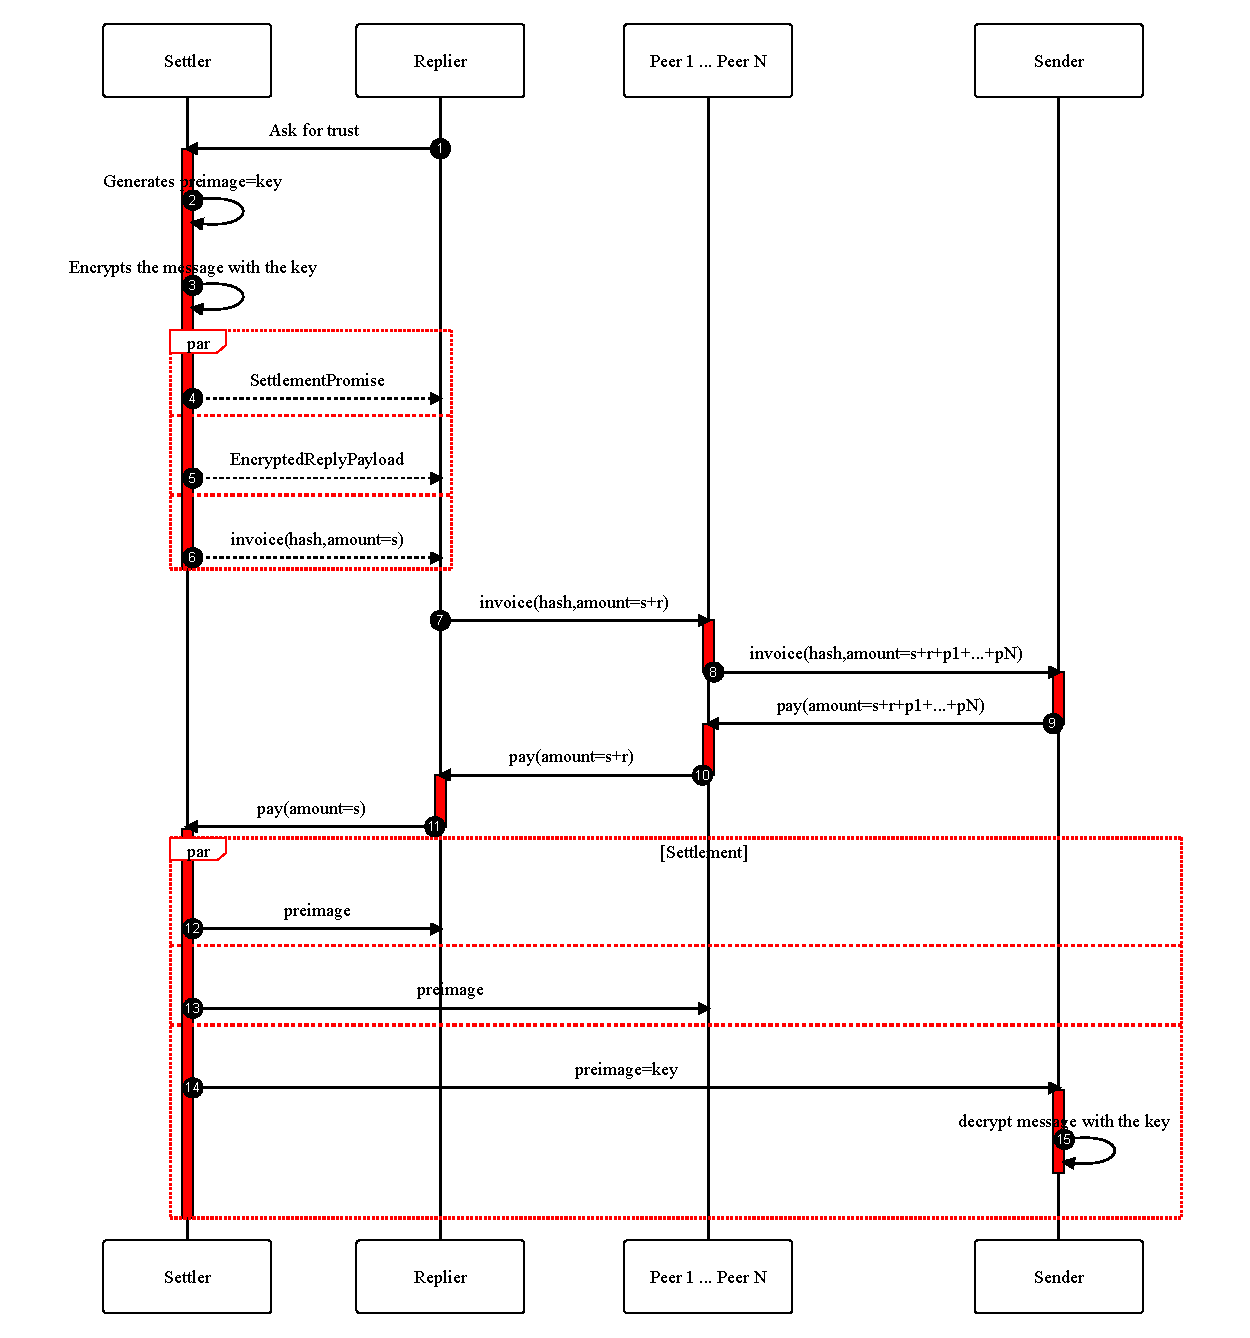
\includegraphics[scale=0.8]{ReplyAndPay.pdf}
	\caption{Reply/Payment/Decryption Sequence}
	\label{fig:replyandpay}
\end{figure}

\begin{figure}
	\centering
	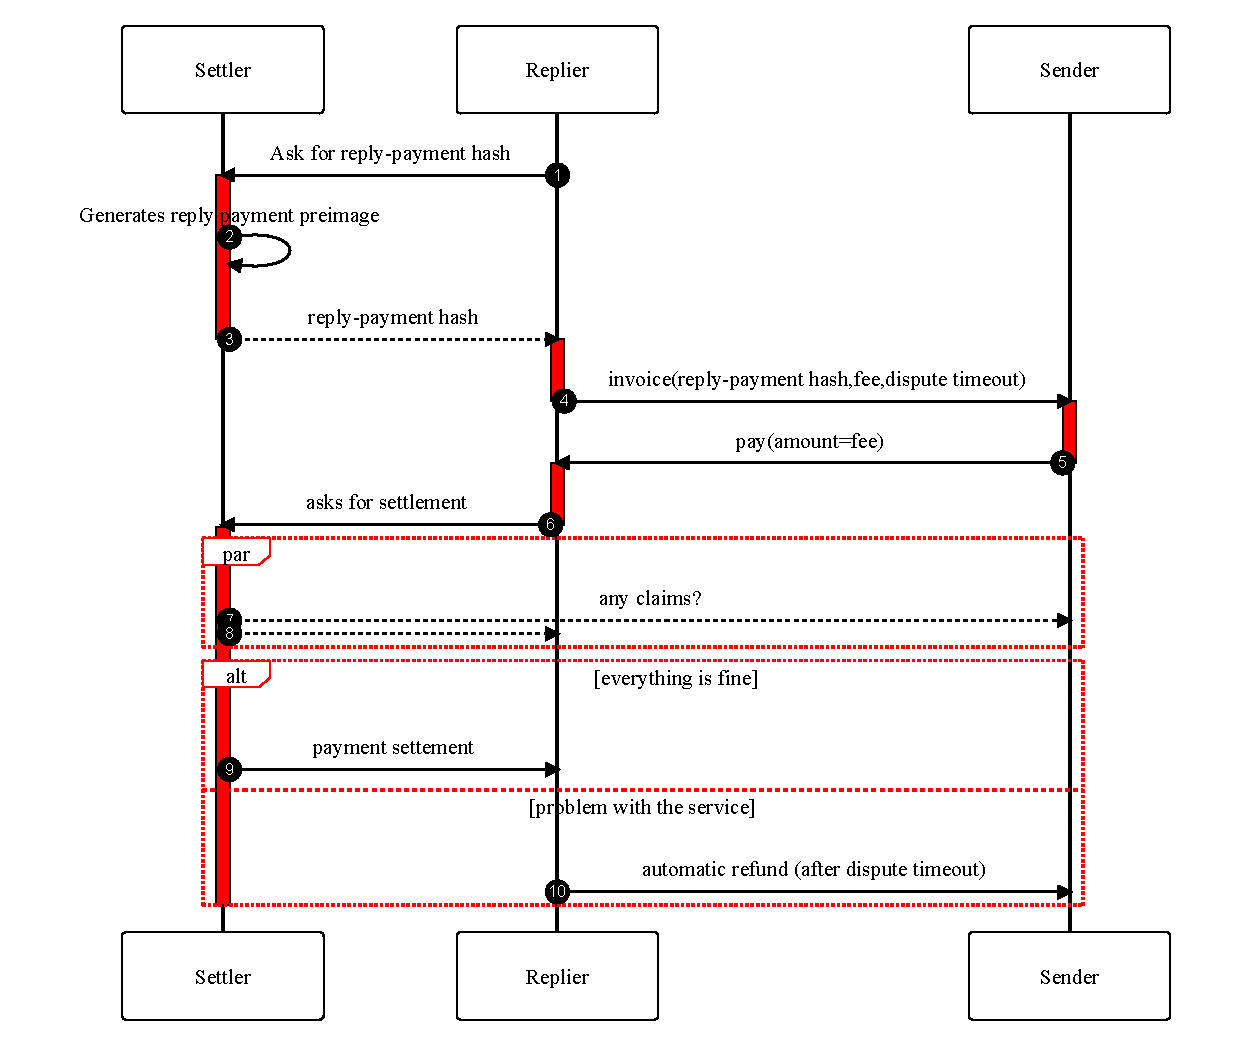
\includegraphics[scale=0.8]{PayForService.pdf}
	\caption{Payment/Settlement Sequence}
	\label{fig:payforservice}
\end{figure}

The last field in ReplyFrame is the network\_invoice. Replier receives the first network\_invoice from the settler, puts network fee on top of this and uses the same network\_payment\_hash as the settler to construct the new invoice and starts listening to its state change. 

Then, while travelling back, each of the middlemen adds its price on top of the invoiced one and replaces the network invoice with the new one, making sure that the network\_payment\_hash remains the same on the entire chain, makes sure that the payment hash of the network invoice is the same as stored in the ReplyPayload, and then starts to listen to its state.

Once it reaches the sender and the sender Accepts the network invoice by paying for it, the chain of acceptances reaches the replier, then it reaches the settler and Once the settler settles its invoice the chain of settlement reaches the sender.

The sender retrieves the preimage and uses it to decrypt the ReplyPayload. Then it uses its own privet key to decrypt the message from the replier.

If one of the settlements fails for some reason, it can break the preimage delivery process, therefore it is important to publish the preimage in an alternative way, it can be done by the settler using its public HTTP endpoint.

[This concludes the protocol.]

\section{Discussion}

\subsection{Distributed Trust}

Payment setters can form a Certification Authority hierarchy. This kind of hierarchy is used commonly in modern internet design however it is based on the idea of trusted 3rd parties. Having Certification Authorities that coexist in a free market helps with the decentralization of trust.

The other possible approach for distributed trust is based on the idea of a track record. Track record means that the specific customer (sender) or gig worker (replier) was already involved in a series of successful transactions. This can be implemented using proof of payments that can be traced back to the specific service being delivered.

The other one is based on the idea of reputation (transitive recommendations), so trustworthy participants are recommending other participants put their reputation on a table.

\subsection{Mobile device connectivity issues}

Creating the mesh of mobile devices requires the ability to establish connectivity between P2P nodes while some of them are behind NAT. The way modern streaming platforms overcome this limitation is based on UDP Holepunching \cite{HolePunching}. Protocols like WebRTC \cite{WebRTC} are well-positioned to solve this issue.

A broken connection between the customer and network or gig worker and network can lead to problems if the routing is based on IP addresses. Next time the mobile network provider connects the device that temporarily lost access, it can assign a different IP address, making the ongoing routing impossible.

\subsection{Attacks}
Here we are discussing common attacks that can be performed on the Gig-gossip network.


\begin{table}  
	\centering
	\begin{tabular}{ll}
		\toprule
		Attack         & Gig-gossip defense \\
		\midrule
		Spam           & POW \\
		DDoS           & POW \\
		Silent         & Multibroadcast > 1 \\
		Chatterbox     & POW \\
		Sybil          & POW \\
		Eclipse        & Multibroadcast >1 \\
		Censorship     & - \\
		Convert Flash  & - \\
		\bottomrule
	\end{tabular}
	\label{tab:attacks}
	\caption{Attacks}
\end{table}


\subsubsection{The Silent Attack}
The adversary tries to distort the distribution of the gossipy nodes to cause propagation failure by failing to respond to the gossip protocol \cite{AdHocNet}. The same behaviour can be just a result of node failure that can happen naturally, especially with mobile devices.

Multibroadcast > 1


\subsubsection{Chaterbox Attack}
A malicious node retransmits repeatedly the same message \cite{AdHocNet}.

\subsubsection{Sybil Attack}
This is the most common form of attack in P2P networks, since creating large numbers of identities is
generally, cheap resource-wise, unless cryptographic puzzles are included as part of joining the system \cite{GossipSub}.

\subsubsection{Eclipse Attack}
This attack can be carried out against a single victim or the whole network. The objective is to
silence the victim by refusing to propagate messages from it or to distort its view by delaying message propagation towards it \cite{GossipSub}.
Here the attack can be performed against a specific Certification Authority

\subsubsection{Censorship Attack}
Sybils seek to establish themselves in the mesh and propagate all messages except those published by the target peer. In contrast to the Eclipse Attack, in the Censorship Attack Sybils appear to behave properly
from all vantage points, but hairpin-drop the victim's messages. The objective of the attacker is to censor the target and prevent its messages from reaching the rest of the network \cite{GossipSub}.

\subsubsection{Covert Flash Attack}
In the Covert Flash Attack, Sybils connect to the network but behave properly for some time in order to build up the score. Then, they execute a coordinated attack whereby they stop propagating messages altogether in an attempt to completely disrupt the network. The attack is difficult to identify before the attackers turn malicious as they behave properly up to that point and build a good profile \cite{GossipSub}.

\section{Reference implementation}
The reference implementation of the Gig-gossip protocol is open-sourced and can be found at \url{https://gig-gossip.org}. The reference implementation is a discrete-time simulation of the protocol running on multiple simulated nodes.

\section{Funding}
If you are interested in funding the Gig-gossip protocol please send Bitcoin (after making sure the paper is not modified - comes from \url{https://gig-gossip.org}) to the following Bitcoin address:

\includegraphics[scale=0.8]{btcaddr.png}

bc1qe092x5mlvh6ul366awydh7kf7397cf8aujw844

\section{Public Key}
This is the Public Key (GPG) of Sonof Satoshi.
\label{gpgkey}
\begin{small}
\begin{verbatim}
-----BEGIN PGP PUBLIC KEY BLOCK-----

mI0EY8pcpgEEAN+bUaEdg+ylWkdNc6U9LNkWb4ii0Neay4kUyU2NntHMlFAZPNSC
wxJ8PlbrQnOGeeGNyfZtjZKTSn0Jor5YT4pHNlubGFj3/BrihJCBRSJ878qO2ct9
4RJXiNADVg1w3jRKRrk1CimmmL7VVK7oFZHd0311+8r/qIT4WNOITydNABEBAAG0
MVNvbm9mIFNhdG9zaGkgPHNvbm9mLnNhdG9zaGlAZG9udHRydXN0dmVyaWZ5Lm9y
Zz6I0QQTAQgAOxYhBIaALVutWo8Bqg5fDYtkf+QR5XMgBQJjylymAhsDBQsJCAcC
AiICBhUKCQgLAgQWAgMBAh4HAheAAAoJEItkf+QR5XMg2PYEAMcEB370PgxAaV+e
Kt458OPymI/rZOWO6Cm9E6BqMdNqNx7d4udxbQYutkUr1xhLmLH1JTxJwFhe3oMv
/3MUjm/VjIYrdnXAhHqvZA3502AyiWEQ66OQ9whj57PY04YYcBZP/NDe4QuoUX9r
b3XzYIeJcqHUNg0zjjQJQ7bU7gcwuI0EY8pcpgEEAK/nkFTpiOiGtUI1RqWD46HA
nH7wTVXy2BVwHefRiDHz2hGgQiHXF6EU8mk9F2SVBjOTBNHGAwvXssT97Y8jiq6i
vJosx7VtolxBEDRL1PFMOH4whwu1rjDg8QR3KPkB3kMcXvD9ZHIB6FspVvhx2/Jk
V+PKLQ0ThhQITxFIKz4nABEBAAGItgQYAQgAIBYhBIaALVutWo8Bqg5fDYtkf+QR
5XMgBQJjylymAhsMAAoJEItkf+QR5XMgRngD/0GbcDFoL8hqppvuBuXBLHJVMLGh
fF/3fZyd1ZkjE+Il/LX5G/WSsLcAm/dmAVd8L1zat3PvdL57RHY06BEE4kdDEo8m
DlZ8SycI1yGaSS8DdGCMaAFLzOxrJgER3NnXxg7BxCfREcUTawq1CEO1QYx/71ib
GoTF/wPiCY/JQ1Ed
=Ei5q
-----END PGP PUBLIC KEY BLOCK-----
\end{verbatim}
\end{small}


\bibliographystyle{abbrv}
\bibliography{references}  

\end{document}
